\documentclass[11pt]{article}
\usepackage[paperwidth=30cm,paperheight=30cm,margin=5mm]{geometry}
\usepackage[T1]{fontenc}
\usepackage{tikz}
\usetikzlibrary{arrows.meta,positioning,fit,backgrounds,calc,shapes.geometric}
\pagestyle{empty}
\tikzset{
  box/.style={draw, rounded corners=2pt, align=center, font=\small, minimum height=9mm, inner sep=4pt, fill=white},
  data/.style={box, fill=blue!8},
  model/.style={box, fill=orange!12},
  outp/.style={box, fill=green!10},
  frozen/.style={box, dashed, font=\small\itshape},
  arr/.style={-{Latex[length=2mm]}, semithick},
  lbl/.style={font=\scriptsize, align=center},
  group/.style={draw, rounded corners=4pt, dashed, gray, inner sep=6pt},
  glbl/.style={font=\scriptsize\itshape, gray, anchor=south west, inner sep=1pt}}
\begin{document}

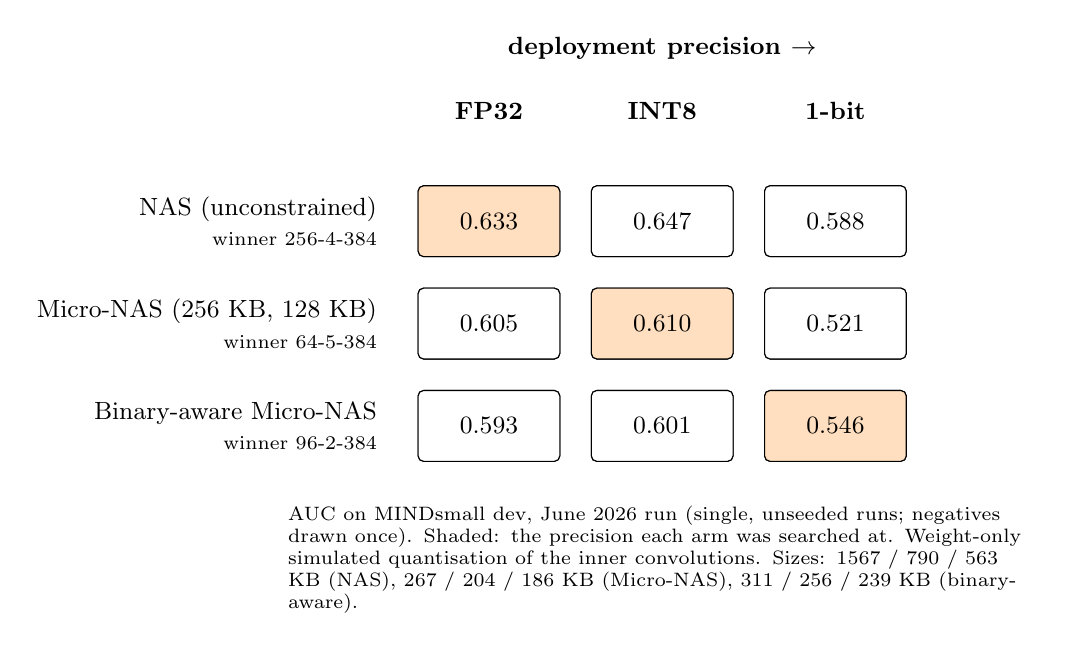
\begin{tikzpicture}[node distance=4mm and 6mm]
  \node[lbl, font=\small\bfseries] at (2.2, 1.2) {deployment precision $\rightarrow$};
  \foreach \j/\p in {0/FP32, 1/INT8, 2/1-bit} {\node[font=\small\bfseries] at (2.2*\j, 0.4) {\p};}
  \foreach \i/\a/\c in {0/{NAS (unconstrained)}/256-4-384, 1/{Micro-NAS (256 KB, 128 KB)}/64-5-384, 2/{Binary-aware Micro-NAS}/96-2-384} {
    \node[font=\small, align=right, anchor=east] at (-1.3, -1.3*\i-1) {\a\\{\scriptsize winner \c}};
  }
  \foreach \i in {0,1,2} \foreach \j in {0,1,2} {
    \node[box, minimum width=18mm, minimum height=9mm, fill=white] (c\i\j) at (2.2*\j, -1.3*\i-1) {};
  }
  \node[box, minimum width=18mm, minimum height=9mm, fill=orange!25] at (c00) {0.633};
  \node[box, minimum width=18mm, minimum height=9mm] at (c01) {0.647};
  \node[box, minimum width=18mm, minimum height=9mm] at (c02) {0.588};
  \node[box, minimum width=18mm, minimum height=9mm] at (c10) {0.605};
  \node[box, minimum width=18mm, minimum height=9mm, fill=orange!25] at (c11) {0.610};
  \node[box, minimum width=18mm, minimum height=9mm] at (c12) {0.521};
  \node[box, minimum width=18mm, minimum height=9mm] at (c20) {0.593};
  \node[box, minimum width=18mm, minimum height=9mm] at (c21) {0.601};
  \node[box, minimum width=18mm, minimum height=9mm, fill=orange!25] at (c22) {0.546};
  \node[lbl, text width=9.5cm, align=left] at (2.2, -5.3) {AUC on MINDsmall dev, June 2026 run (single, unseeded runs; negatives drawn once). Shaded: the precision each arm was searched at. Weight-only simulated quantisation of the inner convolutions. Sizes: 1567 / 790 / 563 KB (NAS), 267 / 204 / 186 KB (Micro-NAS), 311 / 256 / 239 KB (binary-aware).};
\end{tikzpicture}
\end{document}
